\subsection{Определение разрешённых направлений поляроидов}
\begin{enumerate}
    \item Разместим на оптической скамье осветитель
S, поляроид P1 и чёрное зеркало (пластинку чёрного стекла) так, чтобы плоскость падения была горизонтальна. Свет, отражённый от зеркала, рассматриваем сбоку, расположив глаз таким образом, чтобы вблизи оси вращения зеркала можно было увидеть изображение диафрагмы осветителя.
Поворачивая поляроид вокруг направления луча, добьёмся наименьшей яркости отражённого пятна. Оставим поляроид в этом положении
и вращением зеркала вокруг вертикальной оси снова добьёмся минимальной интенсивности отражённого луча.
\begin{figure}[h!]
	  \center{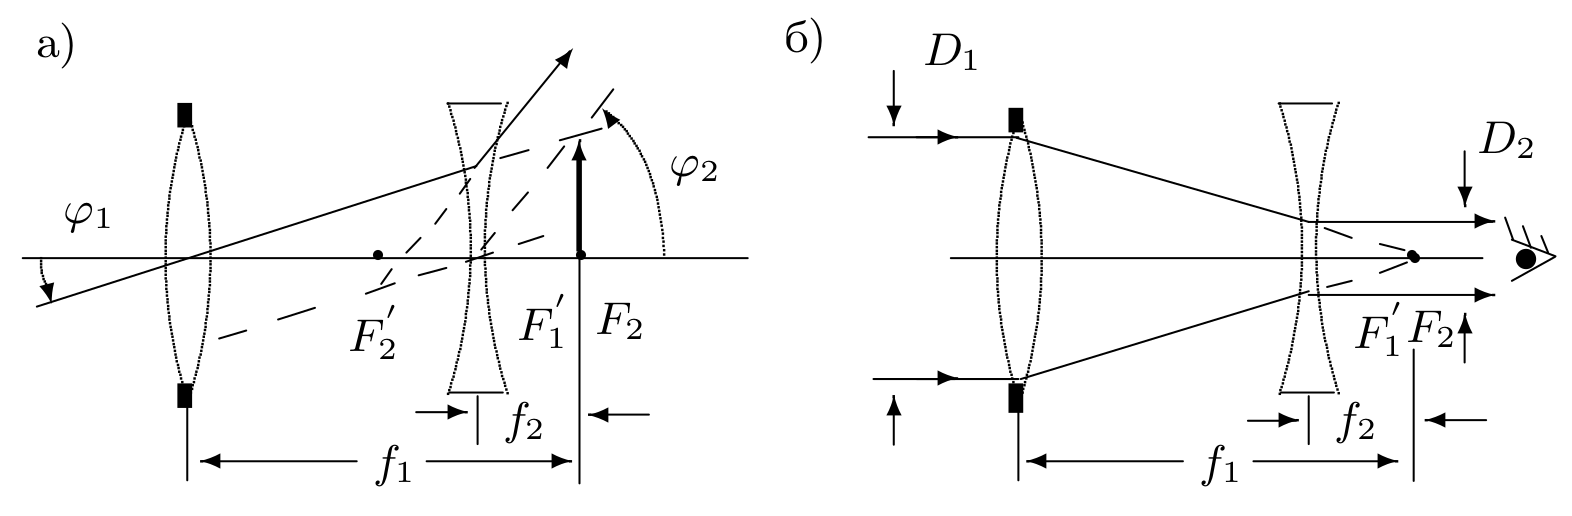
\includegraphics[width=5cm]{5}}
\end{figure}
\par Для первого поляроида разрешённое направление горизонтальное, на лимбе $336^{\circ}$
\item Вместо чёрного зеркала поставим второй поляроид. Скрестим их, определим разрешённое направление второго поляроида - горизонтальная волна, на лимбе $40^{\circ}$
\end{enumerate}
\newpage
\subsection{Определение угла Брюстера для эбонита}
\begin{enumerate}
\item Поставим на скамью вместо чёрного зеркала эбонитовую пластину с круговой шкалой.

\item  Повернем эбонитовое зеркало вокруг вертикальной оси так, чтобы его
плоскость была перпендикулярна лучу, и попытаемся совместить отражённое от эбонита пятно с отверстием осветителя.

\item Установим направление разрешённых
колебаний поляроида P1 горизонтально и найдем угол поворота эбонита
$\varphi_b$, при котором интенсивность
отражённого луча минимальна: его абсолютное значение равно $(304 \pm 2)^{\circ}$

\item Повторим измерения, добавив светофильтр Ф, и сравним результаты - они получились одинаковыми

\item По углу Брюстера рассчитайте показатель преломления эбонита и сравните с табличным.
\begin{center}
    $n = \tg \varphi = \tg (360-304)^{\circ} = 1.4825$
\end{center}
\begin{center}
    $n = (1.5 \pm 0.1)$
\end{center}
Табличное значение показателя преломления эбонита $n = 1.6 - 1.7$

\end{enumerate}
\newpage
\subsection{Исследование стопы}

\begin{figure}[h!]
	  \center{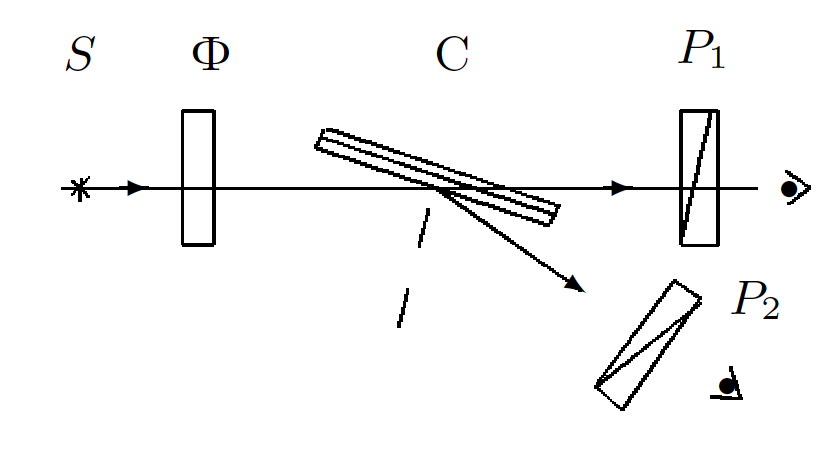
\includegraphics[width=5cm]{6}}
\end{figure}

Поставим стопу стеклянных пластинок вместо эбонитового зеркала
и подберем для неё такое положение, при
котором свет падает на стопу под углом Брюстера.
Осветим стопу неполяризованным светом (снимите поляризатор с оптической скамьи) и, рассматривая через поляроиды свет, отражённый от стопы, определим ориентацию вектора
\textbf{E} в отражённом луче; затем определим
характер поляризации света в преломлённом луче. 
\par Наблюдая прошедший через стопу стеклянных пластинок луч света, убеждаемся, в
том что плоскости поляризации у отраженного и преломленного лучей взаимно
перпендикулярны: Угол на лимбе $P_1 = 328^{\circ}$, $P_2 = 235^{\circ}$. Преломленные лучи горизонтальные, отраженные – вертикальные. Установили, что лучи имеют правый
круговой тип поляризации. 
\newpage
\subsection{Определение главных плоскостей двоякопреломляющих пластин}
Поставим кристаллическую пластинку
между скрещенными поляроидами $P_1$ и $P_2$. Вращая пластинку вокруг направления луча
и наблюдая за интенсивностью света, про
ходящего сквозь второй поляроид, определяем, при
каком условии главные направления пластинки
совпадают с разрешёнными направлениями поляроидов. Повторяем опыт для второй пластинки.

\begin{center}
    Пластина 1 \hspace{1cm} Пластина 2 \\
    $min: 62^{\circ}, 152^{\circ}$ \hspace {1cm} $min: 18^{\circ}, 109^{\circ}$ \\
     $max: 106^{\circ}, 202^{\circ}$ \hspace {1cm} $max: 70^{\circ}, 160^{\circ}$
\end{center}
Минимумы и максимумы интенсивности чередуются через $45^{\circ}$, главные плоскости пластин совпадают с разрешёнными направлениями поляроидов при максимальной интенсивности
\newpage
\subsection{Выделение пластин $\lambda/2$ и $\lambda/4$}
Добавим к схеме зелёный фильтр; установим
разрешённое направление поляроида горизонтально, а главные направления исследуемой пластинки — под углом $45^{\circ}$ к горизонтали. 
\par Пластинка $\lambda/2$ не меняет характер поляризации, при её повороте \textit{меняется интенсивность}, а поляризация остаётся линейной. 
\par Пластинка $\lambda/4$ создаёт сдвиг фаз $\pi/2$ между колебаниями - эллиптическая поляризация. Эта пластинка \textit{не меняет интенсивность} при повороте.
\newpage
\subsection{Определение направлений большей и меньшей скоростей в пластинке $\lambda/4$}

\begin{enumerate}
    \item Поставим между скрещенными поляроидами пластинку чувствительного оттенка ($\lambda$ для зелёного света), имеющую вид стрелки. Световой вектор, ориентированный вдоль направления стрелки, проходит с большей скоростью, перпендикулярный — с меньшей. \par
Установим разрешённое направление первого поляроида горизонтально и убедимся с помощью второго поляроида, что эта пластинка
не меняет поляризацию зелёного света в условиях предыдущего опыта.
\begin{figure}[h!]
	  \center{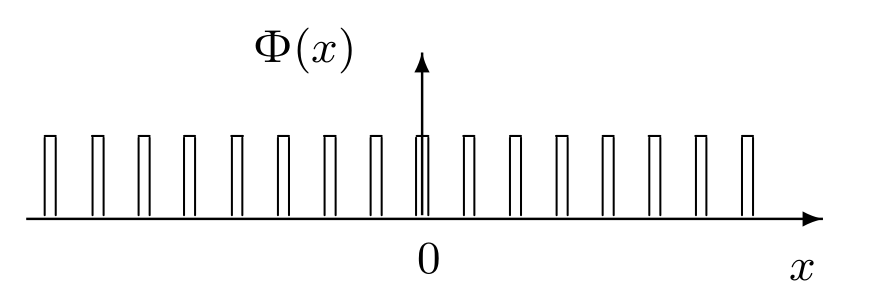
\includegraphics[width=5cm]{7}}
\end{figure}
\item Уберем зелёный фильтр
и поставим между скрещенными поляроидами
пластинку $\lambda$ (стрелка под углом $45^{\circ}$ к разрешённым направлениям поляроидов).
Глядя сквозь второй поляроид на стрелку, убедимся, что она имеет пурпурный цвет - проходят красная и синяя компоненты.
\item . Добавим
к схеме пластинку $\lambda/4$, главные направления
которой совпадают с главными направлениями пластины $\lambda$ и ориентированы под
углом $45^{\circ}$ к разрешённым направлениям скрещенных поляроидов

\item Теперь уберём пластину чувствительного оттенка. После второго поляроида интенсивность минимальная - значит, быстрая ось пластинки направлена горизонтально, направление вращения правое, направление колебаний в первом и третьем квадрантах (разность фаз $\pi/4$). \par
При повороте рейтера со стрелкой на 180◦ вокруг вертикальной оси
цвет стрелки меняется от зелёно-голубого до оранжево-жёлтого.

\end{enumerate}

\newpage
\subsection{Интерференция поляризованных лучей}

Расположим между скрещенными поляроидами мозаичную слюдяную пластинку. Она собрана из 4-х узких полосок слюды, лежащих по сторонам квадрата (две полоски «толщиной» $\lambda/4$ и по одной — $\lambda/2$ и $3\lambda/4$).
\par Вращаем пластинку: изменяется интенсивность света с периодичностью $\pi/4$
\par Вращаем второй поляроид: изменяется (инверсируется) цвет пластинок также с периодичностью  $\pi/4$. Расшифровка пластинки по длинам волн:

    \begin{table}[h]
    \centering
    \begin{center}
    \caption{Результаты наблюдения цвета ячеек}
    \end{center}
    \vspace{0.1cm}
    \label{tab:my_label}
    \begin{tabular}{ |p{2.5cm}|p{2.5cm}|p{2.5cm}|}
 \hline
 $3\lambda/4$ зелёный & $\lambda/2$ пурпурный & $3\lambda/4$ зелёный\\
\hline
 $\lambda/4$ красный & - & $\lambda/4$ красный \\
\hline
 $\lambda$ жёлтый & $3\lambda/4$ синий & $\lambda$ жёлтый \\
\hline
 
\end{tabular}
\end{table}

\newpage
\subsection{Определение направления вращения светового вектора в
эллиптически поляризованной волне}

\begin{enumerate}

    \item Нарисуем эллипс поляризации для вектора \textbf{E}, вышедшего из пластинки, оси X соответствует большая скорость и вышедшие из пластинки синусоиды со сдвигом фаз в 0.25T.
    \begin{figure}[h!]
	    \center{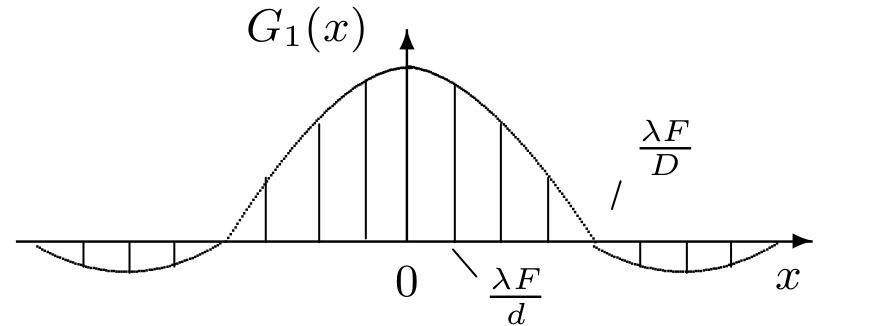
\includegraphics[width=12cm]{8}}
    \end{figure}
    \item  Снова поставим зелёный фильтр,
а за ним между скрещенными поляроидами
$\lambda/4$.
\item Получим эллиптически-поляризованный свет. Для этого установим разрешённое направление первого поляроида под углом $10-20^{\circ}$ к горизонтали так, чтобы вектор \textbf{E} падающего на пластинку света был расположен в первом квадранте.
Установим разрешённое направление второго поляроида вертикально и, вращая пластинку, найдем минимальную
интенсивность света, прошедшего второй поляроид. Вращая второй поляроид, убедитесь, что свет поляризован эллиптически,
а не линейно.
Таким образом, получим эллипс поляризации с вертикально ориентированной малой осью.
\item  Для определения направления вращения светового вектора в эллипсе
установим между поляроидами дополнительную пластинку $\lambda/4$ с известными направлениями «быстрой» и «медленной» осей, ориентированными по осям эллипса поляризации анализируемого света.
В этом случае вектор \textbf{E} на выходе будет таким, как если бы свет прошёл две
пластинки $\lambda/4$: свет на выходе из второй пластинки будет линейно поляризован. Если пластинки поодиночке дают эллипсы, вращающиеся в разные стороны, то поставленные друг за другом, они скомпенсируют
разность фаз, и вектор \textbf{E} на выходе останется в первом
и третьем квадрантах. Если
же световой вектор перешёл в смежные квадранты, значит, эллипсы вращаются в одну сторону. 
\par После второго поляроида интенсивность света максимальна. Значит, две пластины усиливают друг друга, световой вектор перешёл в смежные квадранты, эллипсы вращаются в одну сторону.

\end{enumerate}